\chapter{The Vickrey-Clarke-Groves (VCG) Mechanism}

\subsection*{Motivating Example: Public Good Provision}
Suppose there are $N$ people in a society. Each person has a private value $x_i \in [\alpha, \omega]$ for a new public project (e.g., building a bridge), where $\alpha$ is the minimum possible value (might be negative) and $\omega$ is the maximum. The cost of building the bridge is $c$. 

From a social planner's perspective, the efficient decision is simple:
\begin{itemize}
    \item Build the bridge if $\sum_{i=1}^N x_i \ge c$.
    \item Do not build it if $\sum_{i=1}^N x_i < c$.
\end{itemize}
However, the planner does not know the true $x_i$. If the planner just asks people for their values, they have an incentive to exaggerate (if they want the bridge but don't pay) or understate (if they want to freeride). We need a mechanism to elicit the truth.


\section{The General VCG Framework}
Consider a general direct mechanism $(Q, M)$. 

\defn{Efficient Allocation Rule}{
An allocation rule $Q^*$ is \textit{efficient} if it maximizes the total reported social surplus:
$$Q^*(x) \in \argmax_{Q} \sum_{j = 1}^N Q_j(x) \cdot x_j,$$
subject to feasibility constraints.
\begin{itemize}
  \item If the object is a private good, feasibility requires $\sum_{j=1}^N Q_j(x) \le 1$. 
  \item If it is a pure public good, then everyone consumes it equally: 
  \[
  Q_1(x) = \dots = Q_N(x) \in \{0,1\}.
  \]
\end{itemize}
}

\defn{Social Surplus and VCG Payment Rule}{
  Suppose $Q^*$ is an efficient allocation rule. We define two surplus functions based on the reported types $x$:
  \begin{itemize}
      \item \textbf{Total Maximized Surplus:} 
      \[
      W(x) = \sum_{j=1}^N Q_j^*(x) \cdot x_j.
      \]
      \item \textbf{Surplus of Players Other than $i$:}
      \[
      W_{-i}(x) = \sum_{j\neq i} Q_j^*(x) \cdot x_j.
      \]
  \end{itemize}

  The \textbf{VCG Mechanism} pairs the efficient allocation $Q^*$ with the following payment rule $M_i^*$:
  $$M^*_i(x) = W(\alpha_i, x_{-i}) - W_{-i}(x)$$
  where $\alpha_i$ is the lowest possible type.
}

\rmkb{
\begin{itemize}
  \item \textbf{Intuition: Pricing the Externality}\\
  The VCG payment is exactly the \textbf{social externality} that player $i$ imposes on the rest of the society.
  \begin{itemize}
      \item $W(\alpha_i, x_{-i})$ is the maximum surplus the \textit{other} players could have achieved if player $i$ simply did not exist (or reported the lowest type $\alpha_i$).
      \item $W_{-i}(x)$ is the surplus the \textit{other} players actually end up getting because player $i$ is present and changed the allocation to $Q^*(x)$.
  \end{itemize}
  The difference between what others \textit{could have had} and what they \textit{actually have} is the harm (externality) $i$ causes. VCG forces player $i$ to internalize this exact harm by making them pay it out of pocket.
  \item \textbf{Connection to SPA:}\\
  The Second-Price Auction (SPA) is just a special case of VCG. If you win an SPA, your presence took the item away from the second-highest bidder. The value they lost is exactly the second-highest bid. Therefore, your externality on society is the second-highest bid, which is exactly what VCG/SPA makes you pay.
  \ex[]{
    Suppose there are three bidders for a single object with true valuations $x = (5, 7, 4)$. Let's calculate the VCG payment for the winning bidder (Bidder 2, with value 7):
  \begin{itemize}
      \item If Bidder 2 is absent ($\alpha_2 = 0$), the object goes to Bidder 1 (value 5). The maximum surplus of the others is $W(\alpha_2, x_{-2}) = 5$.
      \item When Bidder 2 is present, the efficient rule allocates the object to Bidder 2. The surplus realized by the \textit{other} players (Bidder 1 and 3) under this allocation is exactly zero: $W_{-2}(x) = 0$.
      \item Bidder 2's payment is $M_2^*(x) = W(\alpha_2, x_{-2}) - W_{-2}(x) = 5 - 0 = 5$. 
  \end{itemize}
  Bidder 2 pays exactly 5, which is the externality they imposed on Bidder 1 by taking the object away.
  }
  \item \textbf{What role does the first term $W(\alpha_i, x_{-i})$ play?}\\
  In the general VCG framework, the first term can be \textit{any} arbitrary function $h_i(x_{-i})$ without violating IC. Because the first term depends ONLY on the reports of others ($x_{-i}$) and a constant ($\alpha_i$), it acts as a constant shift in player $i$'s optimization problem. When player $i$ takes the derivative to maximize their payoff, this term vanishes!  
  
  However, specifically choosing $h_i(x_{-i}) = W(\alpha_i, x_{-i})$, the maximum social surplus achievable \textit{without} player $i$, is known as the \textit{Clarke Pivot Rule}. This specific choice analytically guarantees two crucial properties: 
  \begin{itemize}
    \item \textbf{No Deficit ($M_i \ge 0$):} No one is paid just to participate. 
    
    \textit{Proof:} $M_i^*(x) = W(\alpha_i, x_{-i}) - \sum_{j\neq i} Q_j^*(x)x_j$. The first term is the theoretical maximum surplus the others could achieve on their own. The second term is what they \textit{actually} achieve when $i$ is present. Since the theoretical unconstrained maximum must be greater than or equal to any realized value under constraints, $M_i^* \ge 0$.
    
    \item \textbf{Individual Rationality ($U_i \ge 0$):} No one gets a negative net utility from participating. 
    
    \textit{Proof:} Player $i$'s net utility is $U_i(x) = Q_i^*(x)x_i - M_i^*(x)$. Substituting the VCG payment rule, we can rewrite this as:
    \[
    U_i(x) = W(x) - W(\alpha_i, x_{-i})
    \]
    Here, $W(x)$ is the maximum social pie \textit{with} player $i$, and $W(\alpha_i, x_{-i})$ is the maximum pie \textit{without} player $i$. Because the social planner could always choose to ignore player $i$ and replicate the ``without $i$" outcome, adding a player can never shrink the maximum possible social pie. Thus, $W(x) \ge W(\alpha_i, x_{-i})$, which guarantees $U_i(x) \ge 0$. 
    
    In short, you only pay if your presence ``pivots" the final allocation, but your payment will never exceed the value you personally gain!
  \end{itemize}
\end{itemize}
}

\section{Truth-telling in VCG}

\propp{Truth-telling is a Weakly Dominant Strategy}{
  In the VCG mechanism, reporting the true valuation $x_i$ is a weakly dominant strategy for every player $i$.
}{
  Let $x_i$ be player $i$'s true valuation. Suppose player $i$ reports $z_i$, while the other players report some arbitrary profile $x_{-i}$. 
  
  \rmk{
    Notice that we do NOT assume $x_{-i}$ are truthful. They can be any arbitrary lies. We will show $z_i = x_i$ is optimal regardless of what $x_{-i}$ is. This is the definition of a dominant strategy, which is strictly stronger than a Bayesian Nash Equilibrium.
  }

  Player $i$'s true payoff given these reports is:
  $$
  \begin{aligned}
    \pi_i(z_i | x_i, x_{-i}) & = Q_i^*(z_i, x_{-i})x_i - M_i^*(z_i, x_{-i})\\
    & = Q_i^*(z_i, x_{-i})x_i + W_{-i}(z_i, x_{-i}) - W(\alpha_i, x_{-i})\\
    & = \left[ Q_i^*(z_i, x_{-i})x_i + \sum_{j\neq i} Q_j^*(z_i, x_{-i})x_j \right] - W(\alpha_i, x_{-i})
  \end{aligned}
  $$

  The term in the brackets is exactly the total social surplus evaluated using player $i$'s \textit{true} type $x_i$ and the others' \textit{reported} types $x_{-i}$, under the allocation rule $Q^*(z_i, x_{-i})$. 
  
  By definition, the efficient allocation rule $Q^*$ is the mathematical operator that maximizes the sum of the inputs it is given. Therefore, to make the bracketed term as large as mathematically possible, player $i$ should hand $Q^*$ their true type $x_i$. 
  
  Formally, for any lie $z_i$:
  $$
  \left[ Q_i^*(z_i, x_{-i})x_i + \sum_{j\neq i} Q_j^*(z_i, x_{-i})x_j \right] \le \max_{Q} \left[ Q_i(x_i, x_{-i})x_i + \sum_{j\neq i} Q_j(x_i, x_{-i})x_j \right]
  $$
  The right-hand side is achieved perfectly by reporting $z_i = x_i$. The final term $W(\alpha_i, x_{-i})$ is completely independent of $z_i$, so it cannot be manipulated. Thus, truth-telling maximizes $i$'s payoff for \textit{any} $x_{-i}$.
}

\cor{}{
  $(Q^*,M^*)$ is incentive compatible.
}

\section{VCG Maximizes Revenue Among Efficient Mechanisms}

Let the interim expected payoff (indirect utility) of player $i$ in the VCG mechanism be:
\[
U_i^*(x_i) = \int \left[ Q_i^*(x_i,x_{-i})x_i - M_i^*(x_i,x_{-i}) \right] f_{-i}(x_{-i})\d x_{-i} \equiv q_i^*(x_i)x_i - m_i^*(x_i).
\]

Recall that IC implies $U_i^*(x_i)$ is convex and strictly increasing. 

Suppose $(Q^*, \bar{M})$ is \textit{another} efficient mechanism that is IC. Let $\bar{U}_i$ be its indirect utility function. Because the allocation rule $Q^*$ is identical, the derivative $\bar{U}_i'(x_i) = q_i^*(x_i)$ must also be identical. Therefore, $\bar{U}_i(x_i)$ must have the \textit{exact same shape} as $U_i^*(x_i)$, differing at most by a constant.

Note that in the definition of the Clarke Pivot Rule payment, we carefully included the constant term $W_{-i}(\alpha_i, x_{-i})$ to guarantee that the \textit{lowest type gets exactly zero surplus}: $U_i^*(\alpha_i) = 0$.

\clm{The Individual Rationality (IR) Boundary}{
  For any IC and efficient mechanism to satisfy the IR constraint for all possible types, its utility curve must lie weakly above the standard VCG utility curve.
}{
  We have established that any IC and efficient mechanism yields a utility curve with the exact same shape as the VCG utility curve. By design (the Clarke Pivot Rule), the standard VCG utility curve passes through the origin ($U_i^*(\alpha_i) = 0$). 

  Any alternative mechanism's utility curve $\bar{U}_i$ that is shifted downwards (lying strictly below $U_i^*$) would yield negative utility for the lowest types, directly violating the IR constraint. Conversely, any utility curve shifted upwards (lying strictly above $U_i^*$) perfectly satisfies IR, but implicitly requires the mechanism designer to pay an upfront lump-sum subsidy to the participants.
  \begin{center}
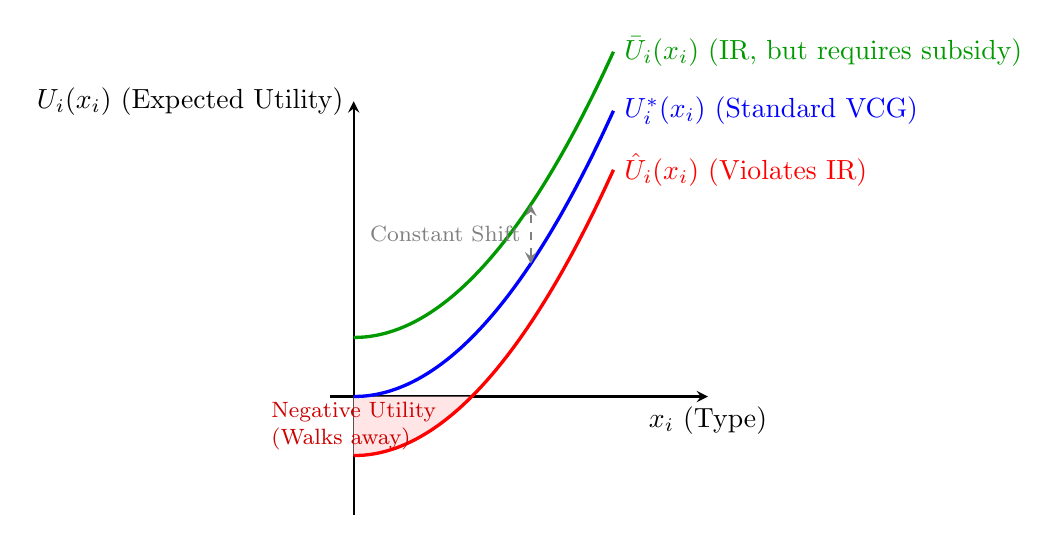
\begin{tikzpicture}[scale=1.5, thick]
  % Axes
  \draw[->, >=stealth] (-0.2, 0) -- (3, 0) node[below] {$x_i$ (Type)};
  \draw[->, >=stealth] (0, -1) -- (0, 2.5) node[left] {$U_i(x_i)$ (Expected Utility)};
  
  % Highlight the IR violation region for the lower curve
  % The lower curve is 0.5*x^2 - 0.5, which crosses x-axis at x=1.
  \fill[red!10] (0,0) -- (0,-0.5) -- plot[domain=0:1, smooth, variable=\x] ({\x}, {0.5*\x*\x - 0.5}) -- (1,0) -- cycle;
  
  % VCG Curve (Base) - Passes through origin
  \draw[domain=0:2.2, smooth, variable=\x, blue, very thick] plot ({\x}, {0.5*\x*\x}) node[right, text=blue] {$U_i^*(x_i)$ (Standard VCG)};
  
  % Upper Curve (Subsidy) - Shifted up
  \draw[domain=0:2.2, smooth, variable=\x, green!60!black, very thick] plot ({\x}, {0.5*\x*\x + 0.5}) node[right, text=green!60!black] {$\bar{U}_i(x_i)$ (IR, but requires subsidy)};
  
  % Lower Curve (Not IR) - Shifted down
  \draw[domain=0:2.2, smooth, variable=\x, red, very thick] plot ({\x}, {0.5*\x*\x - 0.5}) node[right, text=red] {$\hat{U}_i(x_i)$ (Violates IR)};
  
  % Text for the shaded violation region
  \node[align=left, font=\footnotesize, text=red!80!black] at (0, -0.25) {Negative Utility \\ (Walks away)};
  
  % Arrow indicating the constant difference (RET)
  \draw[<->, >=stealth, dashed, gray] (1.5, {0.5*1.5*1.5}) -- (1.5, {0.5*1.5*1.5 + 0.5});
  \node[left, text=gray, font=\footnotesize] at (1.5, {0.5*1.5*1.5 + 0.25}) {Constant Shift};
  
\end{tikzpicture}
\end{center}
}

\rmkb[Why do we ask for IR?]{
  {Could there be a mechanism that is not IR for some regions, but is still reasonable?}
  Yes! It entirely depends on the socio-economic context. Note that in standard mechanism design, we typically assume ``interim" decision-making, where a bidder evaluates IR \textit{after} knowing their own true type $x_i$, but before knowing others'.
  \begin{itemize}
      \item \textbf{Voluntary Participation (Default setting: Auctions, Private Markets):} Here, IR is strictly required for \textit{all} possible types. If $U_i(x_i) < 0$, a bidder of type $x_i$ will simply refuse to participate. Because the designer must ensure the mechanism works regardless of the realized types, the mechanism must universally guarantee $U_i(x_i) \ge 0$.
      \item \textbf{Mandatory Participation (Taxes, Public Goods):} If a government is building a public good or regulating a congestion problem, it has coercive taxing power. You cannot ``opt out" of a society just because the mechanism yields a negative payoff for your specific type. In such compulsory environments, IR is \textit{not} a strict constraint.
  \end{itemize}
}

\propp{VCG Maximizes Revenue Among Efficient Mechanisms}{
  Among all efficient, IC, and IR mechanisms, the standard VCG mechanism maximizes the seller's total revenue $\sum_{i = 1}^{n}m_i$.
}{
  From the previous claim, any alternative efficient, IC, and IR mechanism must provide a utility curve that lies weakly above the standard VCG curve. Providing strictly higher utility to the buyers mathematically necessitates extracting strictly less payment from them. Thus, any deviation from the standard VCG payment rule (such as adding a lump-sum subsidy) strictly decreases the seller's expected revenue.
}

\section{Budget Balance and the AGV Mechanism}

We formally define two expected payment concepts:
\defn{Interim and Ex-ante Expected Payments}{
  Consider a direct mechanism $(Q, M)$ in an environment with $n$ agents, where $M_i(x)$ is the \textit{ex-post} payment exacted from agent $i$ when the reported type profile is $x = (x_i, x_{-i})$. Assume that each agent's type $x_j$ is drawn independently from a type space $X_j$ according to a density function $f_j$. Let $f_{-i}(x_{-i}) = \prod_{j \neq i} f_j(x_j)$ denote the joint density of the other agents' types. 
  
  Define two expected payment concepts corresponding to different information stages:
  \begin{itemize}
      \item \textbf{Interim Expected Payment:} The expected payment of agent $i$ evaluated at the interim stage—conditional on knowing their own realized type $x_i$, but prior to observing the types of other agents. It is defined as:
      \[
      m_i(x_i) = \mathbb{E}_{x_{-i}}[M_i(x_i, x_{-i})] = \int_{X_{-i}} M_i(x_i, x_{-i})f_{-i}(x_{-i})\d x_{-i}
      \]
      
      \item \textbf{Ex-ante Expected Payment:} The expected payment of agent $i$ evaluated at the ex-ante stage—before any agent's type is realized. It is the unconditional expectation of the payment rule over the entire type profile:
      \[
      m_i = \mathbb{E}_{x_i}[m_i(x_i)] = \int_{X_i} m_i(x_i)f_i(x_i)\d x_i = \mathbb{E}_{x}[M_i(x)]
      \]
  \end{itemize}
}

While VCG is elegantly efficient and IC, it is notoriously bad at balancing the budget. It often runs at a deficit (e.g., the mechanism has to inject outside money to pay for positive externalities). 

\ex[VCG Deficit in the Bridge Problem]{
  Consider the 3-person bridge problem with cost $c=10$ and values $x = (5, 6, 2)$. The sum of values is $13 \ge 10$, so the bridge is built. Let's calculate the VCG payments:
  \begin{itemize}
      \item Player 1 ($x_1=5$): Without P1, others value it at $8 < 10$. Not built. P1's payment is $M_1^* = 0 - (6+2-10) = 2$.
      \item Player 2 ($x_2=6$): Without P2, others value it at $7 < 10$. Not built. P2's payment is $M_2^* = 0 - (5+2-10) = 3$.
      \item Player 3 ($x_3=2$): Without P3, others value it at $11 > 10$. Built anyway. P3's payment is $M_3^* = (5+6-10) - (5+6-10) = 0$.
  \end{itemize}
  The total payment collected from all players is $2 + 3 + 0 = 5$. However, the physical cost to build the bridge is $10$. The central planner (or the mechanism) must absorb a massive deficit of $5$ to execute this socially optimal decision!
}

\defn{Budget Balanced}{
A mechanism is \textit{Budget Balanced (BB)} if, for \textit{all} realized profiles $x$:
\[
\sum_{i = 1}^{n}M_i(x) = 0.
\]
}

This is a very strong \textit{ex-post} condition: the agents simply transfer money among themselves under the mechanism.

Naturally, a subsequent question is: \textbf{Does there exist a mechanism that is efficient ($Q^*$), IC, IR, and BB?}

\thmp{Arrow-d'Aspremont-Gerard-Varet (AGV)}{
  There exists an efficient, IC, IR, and BB mechanism if and only if the standard VCG mechanism runs at an ex-ante surplus. That is:
  \[
  \sum_{i = 1}^{n}m_i^* \ge 0.
  \]
}{
  \begin{itemize}
    \item $\implies$:\\
     It is straightforward that if VCG runs at an ex-ante deficit ($\sum m_i^* < 0$), no other mechanism can balance the budget. As discussed, any other IC and IR mechanism must provide a utility curve equal to or above the VCG's curve. Giving everyone more utility means the mechanism must extract even less payment. Thus, the deficit would only widen.
     \item $\impliedby$:\\
     We prove the other direction constructively. This is the celebrated AGV mechanism. Define a new ex-post payment rule $\bar{M}_i(x)$ as:
\[
\bar{M}_i(x) = \underbrace{\left[ m_i^*(x_i) - \frac{1}{n-1}\sum_{j\ne i}m_j^*(x_j) \right]}_{\text{Zero-sum transfers}} + \underbrace{\left[ \frac{1}{n-1}\sum_{j\ne i}m_j^* - \frac{1}{n}\sum_{j = 1}^{n}m_j^* \right]}_{\text{Constant adjustment}}
\]
Summing the payments across all $n$ players:
\[
\begin{aligned}
  \sum_{i = 1}^{n}\bar{M}_i(x) = & \left\{ \sum_{i = 1}^{n}m_i^*(x_i) - \sum_{i = 1}^{n} \left( \frac{1}{n-1}\sum_{j\ne i}m_j^*(x_j) \right) \right\} \\
  & + \left\{ \sum_{i = 1}^{n} \left( \frac{1}{n-1}\sum_{j\ne i}m_j^* \right) - \sum_{i = 1}^{n} \left( \frac{1}{n}\sum_{j = 1}^{n}m_j^* \right) \right\}
\end{aligned}
\]
Notice that $\sum_{i=1}^n \sum_{j \neq i} m_j^*(x_j)$ is simply summing every player's interim payment exactly $n-1$ times. Divided by $n-1$, it precisely cancels out the first term $\sum m_i^*(x_i)$. The first curly brace is strictly $0$. The same combinatorial logic applies to the constants in the second curly brace. Thus, $\sum \bar{M}_i(x) = 0$. The budget balances ex-post.

To see if this new payment rule alters bidding incentives, we must find the new interim expected payment $\bar{m}_i(x_i)$. We take the expectation of $\bar{M}_i(x)$ over all other players' types $x_{-i}$:
\[
\bar{m}_i(x_i) = \mathbb{E}_{x_{-i}}[\bar{M}_i(x)]
\]
Let's pass the expectation operator through the terms linearly:
\begin{enumerate}
    \item $\mathbb{E}_{x_{-i}}[m_i^*(x_i)] = m_i^*(x_i)$ (since it is already an interim function depending only on $x_i$).
    \item $\mathbb{E}_{x_{-i}} \left[ \frac{1}{n-1}\sum_{j\ne i}m_j^*(x_j) \right] = \frac{1}{n-1}\sum_{j\ne i}\mathbb{E}_{x_j}[m_j^*(x_j)] = \frac{1}{n-1}\sum_{j\ne i}m_j^*$. 
    \item The terms in the second bracket are already absolute constants, so their expectation is simply themselves.
\end{enumerate}

Substituting these back in:
\[
\begin{aligned}
  \bar{m}_i(x_i) & = m_i^*(x_i) - {\frac{1}{n-1}\sum_{j\ne i}m_j^*} + {\frac{1}{n-1}\sum_{j\ne i}m_j^*} - \frac{1}{n}\sum_{j = 1}^{n}m_j^*\\
  &  = m_i^*(x_i) - \frac{1}{n}\sum_{j = 1}^{n}m_j^*
\end{aligned}
\]
Note that $\bar{m}_i(x_i)$ only deviates from the standard VCG interim payment $m_i^*(x_i)$ by an absolute constant $\left(\frac{1}{n}\sum m_j^*\right)$. Because the slope of the payment function is unchanged, $(Q^*, \bar{M})$ is perfectly IC.

Furthermore, since the theorem condition explicitly requires the ex-ante surplus to be non-negative ($\sum_{j = 1}^n m_j^* \ge 0$), the constant term we are subtracting is positive. This means the overall payment is reduced (or at worst, unchanged) for every player: $\bar{m}_i(x_i) \le m_i^*(x_i)$. Consequently, players are receiving weakly more utility than in the VCG mechanism, trivially preserving IR.
  \end{itemize}
}

